\section{Epidemiological Model}
\subsection{SIR}
Due to simple dynamics, the population subject to disease spread is divided into three groups: Susceptible (S), Infected (I) and Recovered(R), yielding the Kermack-Mckendrick model (SIR):
\begin{align}
    \dot{S} &= -\beta \frac{ S I}{N_{pop}}\nonumber\\
    \dot{I} &= \beta \frac{S I}{N_{pop}} - \alpha I\\
    \dot{R} &= \alpha I\nonumber
\end{align}
Where $\beta$ is the infection rate in the population, $\alpha$ is the recovery rate and $N_{pop} = S + I + R$ is the total population.

With respect to optimal control of epidemics, both $\beta$ and $\alpha$ can be controllable depending on the situation. $\alpha$ is determined by the expected recovery time of the population, which  may vary depending on the treatment given to the infected. Modeling of the COVID-19 pandemic is usually done by dividing these three groups into multiple subgroups, yielding more complex models which can be fitted to data. However, the work in this project will only be considering the SIR-model with fixed recovery rate $\alpha$.

The main dynamic of interest is the nonlinear dynamic between the susceptible and infected group, which can be controlled by adjusting $\beta$, or in terms of the expected number of infections per individual, $\mathscr{R}_0$:
\begin{equation}
    \mathscr{R}_0 = \frac{\beta N}{\alpha}
\end{equation}

\subsection{Equilibrium Points}
The number of equilibrium points of the system depends on the reproduction number. When $\mathscr{R}_0 < 1$ the disease does not spread fast enough to beat the recovery rate, and will eventually die out. 
\begin{equation}
    \mathscr{E}_0 = (S_\infty, 0, R_\infty)
\end{equation}
This is the disease-free equilibrium, which is the optimal goal for cumulative infection-minimizing control strategies. In the case of a higher reproduction number, another equlilibrium point occurs through bifurcation (Figure \ref{fig:Forward_Bifurcation}). 
\begin{figure}[h]
    \centering
    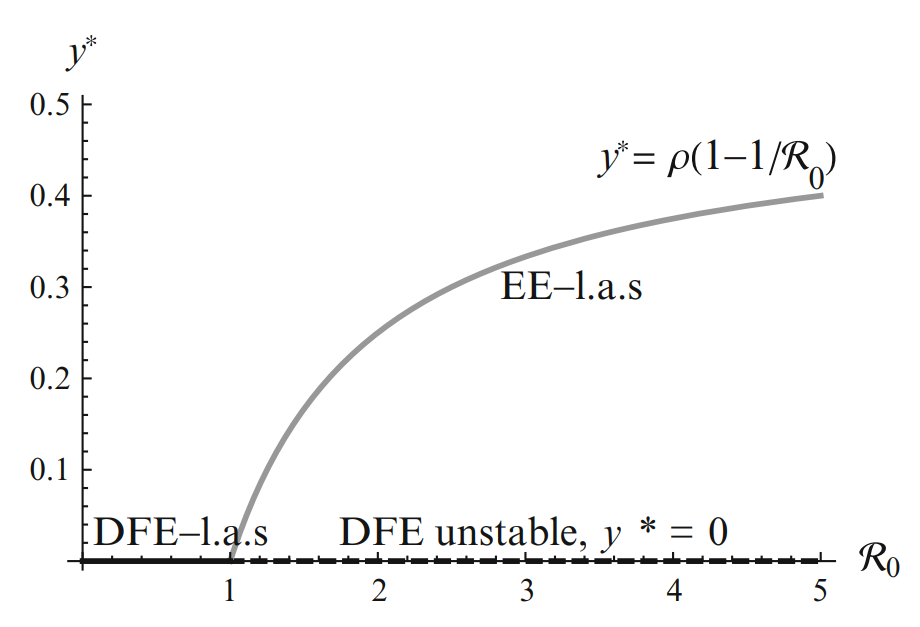
\includegraphics[width = .6\textwidth]{Figures/Bifurkasjonsdiagram_SIR.PNG}
    \caption{Bifurcation-diagram for a dimensionless SIR-model. 
    ($y^*$ is the dimensionless number of infected) [\cite{Martcheva}]}
    \label{fig:Forward_Bifurcation}
\end{figure}

With $\mathscr{R}_0 > 1$ the disease-free equilibrium is unstable. An outbreak will cause temporarily unstable dynamics which will stabilize as the number of susceptibles decrease. The system will converge towards the endemic equilibrium. This equilibrium maximizes the cumulative number of infections.
\subsection{Stability}
\label{ch:SIR_stability}
The local stability in each state can be analyzed with the jacobian of the differential equations:

\begin{equation}
    J = 
    \begin{bmatrix}
    -\frac{\beta I}{N} & \frac{\beta S}{N} & 0\\
    \frac{\beta I}{N} & \frac{\beta S}{N} - \alpha & 0 \\
    0 & \alpha & 0
    \end{bmatrix}
\end{equation}
The three eigenvalues of the jacobian are $\lambda_0 = 0$ and two complex values given by:
\begin{align}
    \lambda_{1,2} &= \frac{\beta(S-I)-\alpha N}{2N}  \pm K\\
\end{align}
The unstable dynamics is given by the real part of the complex eigenvalues, and can be represented by the reproduction number:
\begin{align}
    Re[\lambda_{1,2}] &> 0\\
    \frac{\mathscr{R}_0(S-I)}{N} &> 1
\end{align}
The most unstable achievable dynamic occurs when $\mathscr{R}_0 = \mathscr{R}_{0, max}$ and $\max_{S, I} (S-I)$. Since $S$ is monotonically decreasing, this will occur at $(S, I, R) = (S_0, I_0, R_0)$.

\subsection{Control strategies}
Reduction of the number of infected can be achieved using different strategies, including vaccination, quarantine and social distancing measurements. The different types of mitigation will affect the groups in the SIR model differently.  

\subsection{Social Distancing}
In addition to minimization of the total number of infections, a penalty to the strictness of the social distancing policies can be introduced, resulting in the following minimization problem:
\begin{equation}
    \min_{w} \Phi(w) = \min_{u = [u_0, \dots, u_k]} \int_{t=0}^{T_{end}} I^2(t) - W_u u^2(t)
\end{equation}

Where $u$ is given as the reproduction number $\mathscr{R}_0$ in this case. The constant relationship between $N_{pop}, \alpha$ and $\beta$ makes $\mathscr{R}_0$ and $\beta$ only differ in scaling. 

\subsection{Vaccination}
Vaccination can be implemented as a flow rate from the susceptible to the recovered group. 
\begin{align}
    \dot{S} &= -\beta \frac{SI}{N_{pop}} - (\alpha_v S\mbox{ or }  \alpha_v)\\
    \dot{R} &= \alpha I + \alpha_v S
\end{align}
Increased vaccination will be represented as a positive contribution to the objective function. 
\begin{align}
    \begin{split}
    \min_{w} \Phi(w) &= \min_{u = [u_0, \dots, u_k]} \int_{t=0}^{T_{end}} I^2(t) + W_u u^2(t)\\
    u &= \alpha_v
    \end{split}
\end{align}


\subsection{Isolation}
Putting infected individuals in quarantine eliminates their potential infectiousness, and can be viewed as transfering them over to the recovered group.
\begin{align}
    \dot{I} &= \beta \frac{SI}{N_{pop}} - (\alpha + \alpha_q) I\\
    \dot{R} &= (\alpha + \alpha_q) I
\end{align}

Increased quarantine measures will be represented as a positive contribution to the objective function.
\begin{align}
    \begin{split}
    \min_{w} \Phi(w) &= \min_{u = [u_0, \dots, u_k]} \int_{t=0}^{T_{end}} I^2(t) + W_u u^2(t)\\
    u &= \alpha_q
    \end{split}
\end{align}
Quarantine rate range is more difficult to estimate due to underreporting, self-isolation and asymptomatic individuals. 

\subsection{Problem Parameters}
\label{ch:Problem_Parameters}
For social distancing the reproduction number will be lower-bounded by the lowest estimated value from FHI's national report on the spread of covid-19 in Norway (03/02-21,[\cite{FHI_report}]).$\mathscr{R}_0$ will be upper bounded approximately to one of the highest estimates for countries worldwide ([\cite{France_high_R0}]). $\alpha$ will be fixed according to the expected time spent in the infectious class[\cite{Infectious_Period}]. 
\begin{align}
\alpha &= \frac{1}{9[\text{days}]} \approx 0.11\\
\mathscr{R}_0 &\in [0.5, 6.5]
\end{align}

The default time horizon for the control problems is set to $t \in [0, 28] [\text{days}]$. The population size is set approximately to Norways total population ($N_{pop} = 5.3\times 10^6$), and the initial number of infected is set to $2000$. 

As of 24/02-21, a rough average of the vaccination rate is $\approx 2400$ individuals per day over the past five weeks in Norway. The vaccination rate may be modeled as proportional to $S$, or a flat parameter rate. 
\begin{equation}
    \alpha_v \in [0, 3\times2400]
\end{equation}

An arbitrary range of $\alpha_v \in [0, 1], \alpha_q \in [0, 1]$ is set to view the effect of the proportional terms.

Unless stated otherwise, the economical weighting factor $W_u$ is set to a value where the cost-reduction of $u(t)$ is large enough to make an impact on the control strategy. For social distancing it can be chosen according to equation \ref{eq:Wu_sc}.

\begin{equation}
    W_u = \frac{N_{pop}^2}{k(u_{max}-u_{min})^2}
    \label{eq:Wu_sc}
\end{equation}



